\documentclass[12pt,twoside]{jsarticle}

%%%%% ----- パッケージ ----- %%%%%
\usepackage[dvipdfmx]{graphicx}
\usepackage[deluxe]{otf}
\usepackage{fancyhdr}
\usepackage{titlesec}
\usepackage{ascmac}
\usepackage{listings}

%%%%% ----- 余白設定 ----- %%%%%
\setlength{\textheight}{\paperheight}
\setlength{\topmargin}{1cm}
\setlength{\headsep}{1cm}
\addtolength{\topmargin}{-\headheight}
\addtolength{\topmargin}{-\headsep}
\addtolength{\textheight}{-60truemm}

%%%%% ----- コマンド設定 ----- %%%%%
\newcommand{\figref}[1]{Fig. \ref{#1}}
\newcommand{\tabref}[1]{Table. \ref{#1}}
\newcommand{\eref}[1]{式(\ref{#1})}
\renewcommand{\figurename}{Fig.}
\renewcommand{\tablename}{Table}
\renewcommand{\postsectionname}{章}
\titleformat*{\section}{\huge\bfseries}

%%%%% ----- コード入力設定 ----- %%%%%
\lstset{
basicstyle={\ttfamily\small},
frame=tRBl,
framesep=10pt,
breaklines=true,
linewidth=12cm,
lineskip=-0.5ex,
tabsize=2
}

%%%%% ----- 表紙設定 ----- %%%%%
\makeatletter
\renewcommand{\title}[0]{\large 日本語のタイトル}
\newcommand{\etitle}[0]{\Huge English Title\\\vspace{3mm} 2段目はここ}
\renewcommand\maketitle{
\vspace{5mm}
\begin{center}
 {\large 平成??年度 卒業研究論文}
 %\vspace{1cm} \\
 \vfill
 {\bf \etitle} 
 \vspace{5mm} \\
 {\title}
\end{center}
	\begin{flushright}
		% {\large 平成??年度 卒業研究論文}
		% \vspace{1cm} \\
		% {\bf \etitle}
		% \vspace{5mm} \\
		% {\title}
		\vfill
		{\Large \today}
		\vspace{1cm} \\
		{\large 茨城工業高等専門学校~~電子情報工学科}
		\vspace{3mm} \\
		{\huge {\it NAMAE~~MYOJI}}
		\vspace{3mm} \\
		{\large 苗字~~~名前}
		\vspace{1cm} \\
		{\large {\it Supervised~by~Kei~KOGAI}}
		\vspace{1mm} \\
		{\large 指導教員~~~~~小飼~~敬~~~教員}
	\end{flushright}
}
\makeatother

%%%%% ----- ヘッダとフッタ ----- %%%%%
\fancyhead{}
\fancyhead[Ro]{\rightmark}
\fancyfoot{}
\fancyfoot[Ro]{\thepage}
\fancyfoot[LE]{\thepage}

%%%%% ----- ここから内容 ----- %%%%%
\begin{document}

%%%%% ----- 表紙 ----- %%%%%
\pagestyle{plain}
\maketitle
\thispagestyle{empty}
\newpage
\thispagestyle{empty}
\ 
\newpage

%%%%% ----- 目次 ----- %%%%%
\pagestyle{fancy}
\pagenumbering{roman}
\tableofcontents
\newpage

%%%%% ----- 目次が奇数ページの場合はここのコメントを外す ----- %%%%%
%\fancyhead[Ro]{}
%\fancyhead[RE]{\rightmark}
%\fancyfoot[Ro]{}
%\fancyfoot[LE]{}
%\fancyfoot[RE]{\thepage}
%\fancyfoot[Lo]{\thepage}

%%%%% ----- ここから本文 ----- %%%%%
\pagenumbering{arabic}

%%%%% ----- 解説を入れておいたよ ----- %%%%%
\section {LaTeXの解説 基礎}
\vspace{10pt}
文章はここに書く.
普通の改行では改行されない.
バックスラッシュ二つで改行される\\
段落を変える場合は\par
次の文章は一文字落ちる.
改行二つでも段落が変わる


引用したいときは\cite{タグをここに書く}で番号を付与できる(要二回実行).引用に関しては参考文献も参照してほしい.
\par
\vspace{5pt}
段落を変える時はvspace{5pt}で行間を空けると綺麗に見える
\clearpage
\section {LaTeXの解説 サブセクション}
\vspace{10pt}
\subsection{サブセクション名をここに書く}

%\vspace{5pt}
サブセクションの下にvspaceで余白を作る事で狭苦しくならない.
\subsubsection{さらにもう一段階作りたい時はこんなかんじ}
%\vspace{3pt}
サブサブの下に余白を入れるかどうかは好みによると思う.テンプレ作者は入れる派.これより細かいセクションはできない.そこまで細かくすると却って見づらくなってしまう.

\begin{itemize}
 \item 箇条書きはこんなかんじ
 \item いくらでも増やせるよ
       \begin{itemize}
	\item 入れ子もできるよ
	\item さすが\LaTeX だね
	      \begin{itemize}
	       \item ちなみに\TeX とか様々なコマンドが存在するよ
	       \item 特に数式のコマンドは人によってはたくさん使うんじゃないかな
	      \end{itemize}
	\item endで入れ子脱出.
       \end{itemize}
 \item 入れ子にしたらendを忘れずに.
\end{itemize}
画像の挿入は次のセクションで扱っているよ

\subsection{二つ目のセクション名}
%\vspace{5pt}
セクションは多ければ多いほど良いという訳では無いけれど,目次が豪華になってそれっぽく見えるよ.でもサブサブセクションは目次には反映されないよ.
%\par \vspace{5pt}

もしなんらかの理由(配置とか?)でページを変えたい場合は,
\newpage
で次のページに移るよ.画像を表示している時の改ページは注意点があるよ.それも次のセクションで扱うよ.
\par \vspace{5pt}
もし文章を枠で囲いたい時は...
\vspace{5pt}
\begin{itembox}[l]{ここに題名を書こう}
ここに内容を書こう
\end{itembox}
\par \vspace{5pt}
改行を忘れずに!

\subsection{追加説明したい時}
%\vspace{5pt}
なんらかの理由(配置とか?) ... あまりかっこよく無い!

%\par \vspace{5pt}
なんらかの理由\footnote{配置とか?} ... 論文っぽい!こっちの方がオススメ.
\clearpage
\section {LaTeXの解説 画像}
\vspace{10pt}
\subsection{画像の挿入}
%\vspace{5pt}
画像を挿入したい時は,このファイルの最後にあるセットを組み込んでね.

\subsection{使用例}
%\vspace{5pt}
進捗が一向に進まない...そんな友人に送るべき画像をFig.\ref{fig:class}に示す.この画像を見せた時の反応は以下の5種類に分けられる.

\begin{itemize}
 \item 顔は笑いながらキレる
 \item 無表情でキレる
 \item 眉を吊り上げてキレる
 \item 無言でキレる
 \item 殴ってくる
\end{itemize}

画像を入れた際の改ページは注意が必要.改ページする前に全ての画像を出力したい時は,\ newpage \footnote{空白を開けているのはコマンドを実行して欲しく無いため}ではなく\ clearpage を使う.\ newpage を使用した場合,まだ出力されていない画像は改ページ後に出力される.

%%%%% ----- ここから画像挿入コマンド ----- %%%%%
\begin{figure}[tb]
\centering

\includegraphics[width=12cm]{fig/class.pdf} %ここに画像ファイルの名前を拡張子ごと入力,12cmは画像の大きさ
\caption{Class diagram} %題名はここ
\label{fig:class} %自由に名前をつけられる.図番号を呼び出す際に使う
\end{figure}
\clearpage
\section {LaTeXの解説 その他}
\vspace{10pt}
%\vspace{10pt}
\subsection{コードの埋め込み}
もしコードを埋め込みたいなら...

\begin{lstlisting}
#include <stdio.h>
int main(void)
{
	printf("Hello, World !\n");
	return 0;
}
\end{lstlisting}
この中では改行も含めて書いたままが出力されるよ.

\subsection{表記の統一}
拡張現実と拡張現実感など,表記ゆれに気をつける.気をつけると気を付けるなど漢字にも注意.二日間と2日間もよくある表記ゆれ.また語尾は~だ,~である調で書く.\footnote{ただし謝辞は~です~ます調で書かれることが多い.}

\subsection{長音符の扱い}
四字以上で最後が長音符だった時,長音符は省略する.\\例
\begin{itemize}
 \item NG:プリンター OK:プリンタ
 \item NG:キャラクター OK:キャラクタ
 \item NG:メンバー OK:メンバ
\end{itemize}
この間違いは多発するので特に注意.

\subsection{句読点}
句読点の打ちすぎに注意.例えば,こんな感じで,多用すると,とても,読みづらい.\\
読点が多くなったら文の前後入れ替えや語尾の変更などでいい感じに整えよう.

\newpage
ここから先はテンプレート作成者田村の論文です.参考になるかは分かりませんが...\\
今まで1年間研究を頑張ってきたと思いますが,論文作成は1年間の総仕上げです.これからが本番と言っても過言ではないでしょう.論文は計画的に.2日前には担当教員に提出できるように!\footnote{ちなみに作成者は提出日に寝坊して3時間遅れで提出しました}

%\par \vspace{5pt}
最後の謝辞に少しだけ注釈を入れてあります.消去するのを忘れないように気をつけて下さい.
%\par
%\vspace{10pt}

作成日 2017年 2月 27日\footnote{2月28日が卒研発表日でした} 小飼研 田村 優
\clearpage

%%%%% ----- はじめに ----- %%%%%
% [intro.tex]というTEXファイルを用意する
\section{はじめに}
\vspace{10pt}
2016年は「VR元年」とも呼ばれるほどにVRの発展が目覚ましかった.VR,すなわち仮想現実感は被験者に完全な仮想の視界を提供する技術であり,被験者の視界は完全に遮られ代わりに新しい視界を与えられる\cite{VR}.
今まで以上にリアリティの高い経験を得ることができることから世界中の注目を集め,今では一つの分野として成長を続けている.

%\par
%\vspace{5pt}
また,VRと似た分野にARというものがある.AR,すなわち拡張現実感とは,被験者の視界を完全には遮らず,普段の視界を保ったまま新たな情報を提供する技術である.拡張現実感と仮想現実感は名前こそ似ているがその実態は全く異なり,使われている技術や想定されている使用用途など様々な点で違いがある.

%\par
%\vspace{5pt}
仮想現実感は視界を完全に遮るため自身の移動に大きな制限が掛かってしまう.その為殆どの場合その場から動いて使用するような想定はされていない.これは据え置き型のゲームとの相性がとても良く,現在も仮想現実感を用いた据え置き型ゲームの市場は拡大しつつあると言える\cite{VRnews}.

%\par
%\vspace{5pt}
拡張現実感は仮想現実感とは違い現実の視界が保たれているため,移動しながらの使用も可能である.また移動しながら使用することを想定したアプリケーションも開発されてきた\cite{ARapp}.

%\par
%\vspace{5pt}
ここで仮想現実感と拡張現実感の違いのもう一つ,すなわち使われている技術について注目してみると,意外なほどに異なっている.仮想現実感では3Dグラフィックス,頭の向きを測るための加速度計測などが中心に使われる.しかし拡張現実感では3Dグラフィックスに加え画像認識を用いている.つまり向いている方向を判断する技術が全く異なるのだ.

%\par
%\vspace{5pt}
今までに挙げた仮想現実感と拡張現実感の特徴をまとめると,仮想現実感は趣味や娯楽方面でとても有用だということがわかる.また拡張現実感は仕事や生活の効率化に有用だということがわかる.しかし,拡張現実感は仮想現実感に比べ世間の注目度や浸透度などにおいて遅れをとっていると言える.

%\par
%\vspace{5pt}
何故,拡張現実感はそこまで仮想現実感に比べ発展していないのだろうか?著者はこの疑問に対する回答及び解決案を提示することにした.
\clearpage

%%%%% ----- 開発経緯 ----- %%%%%
% [story.tex]というTEXファイルを用意する
\section{開発経緯}
\vspace{10pt}
\subsection{何故発展しないのか}

%\vspace{5pt}
\subsubsection{要因予想}
前章で拡張現実感の現状を述べた.少ないながらも拡張現実感を実現させるためのライブラリは提供されているが,何故ここまで拡張現実感は広まっていないのか?著者はその要因を以下のように予想した.

\begin{itemize}
 \item 興味を持つ人が少ない
 \item 拡張現実感が何かを知らない
 \item 拡張現実感を使う,という発想が無い
 \item 実装することで得られるメリットが少ない
 \item そもそも実装が難しい
\end{itemize}

ほかにも様々な要因があると思われるが,上に挙げただけでも拡張現実感が普及しない理由としては十分だと言えるだろう.
\par \vspace{5pt}
この要因に対して,解決案をそれぞれ考えることにした.

%\vspace{5pt}
\subsubsection{解決案}
先程述べた要因に対して,それぞれ解決案を考えてみた結果を以下に示す.
\begin{itemize}
 \item 興味を持つ人が少ない
 \item 拡張現実感が何かを知らない
       \begin{itemize}
	\item 拡張現実感を用いたイベント等で興味を持ってもらう
	      \begin{itemize}
	       \item 例) スマートフォンでかざしてみると様々な立体映像が見られる等
	      \end{itemize}
       \end{itemize}
       \vspace{10pt}
 \item 拡張現実感を使う,という発想が無い
 \item 実装することで得られるメリットが少ない
       \begin{itemize}
	\item 拡張現実感を用いることで得られるメリットをPRする
	      \begin{itemize}
	       \item 例) 拡張現実感を用いたシステム等からどれだけ付加価値があるか調べ,公表する
	      \end{itemize}
       \end{itemize}
 \item そもそも実装が難しい
       \begin{itemize}
	\item 開発しやすい環境を構築する
       \end{itemize}
\end{itemize}

\newpage
上記より,上から2つに関してはイベントなどで拡張現実感を使うというもので,まずは拡張現実感というものを知ってもらおうという案である.続く2つは,メリット等が分かっただけでは最後の``開発の難しさ''に直面し,これだけでは意味がない.
\par \vspace{5pt}
結果,まず取り組むべき要因は``拡張現実感に興味を持ってもらう''と``開発の難易度を下げる''だと考えた.

%\vspace{5pt}
\subsection{解決案}
上に挙げた要因より,``拡張現実感に興味を持ってもらう''と``開発の難易度を下げる''が最優先ではないかと考えた.そしてこの二つを解決するためには,以下の案がとても効果的ではないかという結論に至った.\par

\vspace{5pt}
\begin{itembox}[l]{解決案の提案}
拡張現実感を初めて体験する人に向けた簡易的なライブラリの制作
\end{itembox}
\par
\vspace{5pt}

また,使用するデバイスはAndroidを選択した.理由はカメラと画面が一体化しており,直感的な操作ができるから,また今後の発展性が大きく望めるからである.
\par \vspace{5pt}
しかし,プログラミング初心者向けの言語であるProcessing\cite{Processing}などと違い,Androidは複雑で高機能,どちらかといえばプログラミングに慣れた人でないと扱うのが難しい言語である.実際``Hello,World!''を表示する事はそこまで難しくないが,そこから新しい機能を追加するとなると途端に難しくなってしまう.ライブラリの追加方法やその利用方法などもある程度Android開発を経験している開発者向けの説明が殆どで,一から詳しく解説しているドキュメントはとても少ない.
\par \vspace{5pt}
Androidは拡張現実感を体験するにはとても良いが,開発が難しい.そこで,``とりあえず拡張現実感を体験してみよう''をテーマにしたAndroid向けライブラリの作成をしようと考えた.
\clearpage

%%%%% ----- 設計 ----- %%%%%
% [plan.tex]というTEXファイルを用意する
\section{設計}
\vspace{10pt}
\subsection{コンセプト}
今回作成するライブラリのコンセプトを以下に示す.

\begin{itemize}
 \item 対象者
       \begin{itemize}
	\item Androidアプリケーション開発初学者
       \end{itemize}
 \item 想定している使用目的
       \begin{itemize}
	\item 中・高生等を対象にしたセミナー
	\item Computer Graphics(CG)の授業や実験
	\item 企業等での3DCGを用いたAndroidプログラミングの学習
       \end{itemize}
 \item ライブラリの特徴
       \begin{itemize}
	\item 関数名や変数名を明瞭化
	\item 役割ごとにクラスを分け,各クラスの役割を明瞭化
	\item 拡張しやすい構成にする
	\item MainActivity\footnote{Androidアプリケーションを実行した時,一番最初に実行されるメソッド}はできるだけ最小限の構成に
       \end{itemize}
\end{itemize}

%\vspace{5pt}
\subsection{開発環境}

%\vspace{5pt}
\subsubsection{Android開発環境の現状}
現在,Androidアプリケーションの開発環境は以下の二つが主流である.
\begin{itemize}
 \item Eclipse\cite{Eclipse}
       \begin{itemize}
	\item Javaをはじめとするいくつかの言語に対応している統合開発環境である.Androidが登場してすぐの頃はEclipseでの開発が主流だった.
       \end{itemize}
 \item AndroidStudio\cite{AndroidStudio}
       \begin{itemize}
	\item Androidを開発しているGoogle社が提供しているAndroid統合開発環境である.初期のAndroidStudioは動作が不安定だった為しばらくはEclipseが使われていたが,最近はアップデートを繰り返し安定性が増してきている.
       \end{itemize}
       現在はEclipseからAndroidStudioに移りつつあると言える.しかし依然Eclipseで開発をする人が多い事も事実である.
\end{itemize}

\newpage
現状を踏まえて以下の環境で開発する事にした.
\begin{itemize}
 \item OS : Mac OS X Yosemite\cite{Yosemite}
       \begin{itemize}
	\item 動作の安定性,今後iOS版\footnote{iOSではSwiftと言われる言語を使用しており,開発は今の所Macでないと不可能である}の開発をする可能性などを考慮し,Mac miniを使用した.
       \end{itemize}
 \item 開発環境 : AndroidStudio 2.2.2
       \begin{itemize}
	\item 近年の開発環境の遷移を踏まえて,これからのスタンダードと考えられるため選択した.
       \end{itemize}
 \item 使用ライブラリ : ARToolKit version 5.3.1
       \begin{itemize}
	\item Androidの最新バージョンに対応している他,様々なプラットフォームに対応している為今後の展開を踏まえ選択した.
       \end{itemize}
 \item 実行端末 : Nexus 9\cite{Nexus9}
       \begin{itemize}
	\item Android 7.0 が動作するNexus 9 をARアプリケーションの実行端末として使用した.
       \end{itemize}
\end{itemize}

%\vspace{5pt}
\subsection{構造}
構造の明瞭化を図る為クラスを以下のように分割し,利用者が使用するクラス,ライブラリに格納できないクラスを除き全てライブラリに格納する.クラス図をFig.\ref{fig:class}に示す.またライブラリ化する事によって改変によるエラーを防ぎ,明瞭なコードになるよう促す.

%\vspace{5pt}
\subsubsection{Appモジュール}

\begin{itemize}
 \item MainActivity
       \begin{itemize}
	\item 簡易化する為,親クラスを変更しSetupを呼び出すだけとなっている.
       \end{itemize}
 \item Setup
       \begin{itemize}
	\item ここではライブラリに格納できない設定を行うクラスである.初学者には難しい設定や変更する必要のないメソッド等が格納されている為,ライブラリと共に提供されるクラスである.使用者は提供されたSetupクラスに指定の変更を加え,MainActivityと同じパッケージに入れるだけで実装が完了する.
       \end{itemize}
 \item AR
       \begin{itemize}
	\item 実際にARで表示したい物体の設定をするクラスである.簡易化を図る為,表示できるのはBoxのみである.Boxの大きさ,色,位置,角度,対応するARマーカーを登録するクラスで,使用者はここを変更する事で様々な変化を作る事ができる.
       \end{itemize}
\end{itemize}

%\vspace{5pt}
\subsubsection{ライブラリ}

\begin{itemize}
 \item Draw
       \begin{itemize}
	\item ARマーカの検出,及びBoxの表示をする処理が入っている.複数のマーカに反応させる場合や時間が経つにつれて変化を起こしたい場合,ここの処理を変更しないといけない.
       \end{itemize}
 \item ARSimpleApplication
       \begin{itemize}
	\item ARToolKitライブラリを使用する際にAppモジュールに追加しないといけなかったが,ライブラリ内に移動する事で処理の明瞭化を図る.
       \end{itemize}
 \item Cube
       \begin{itemize}
	\item 与えられた情報から色情報付きのBoxを生成するクラスである.ここを変更する事でBox以外の物体を表示できるが,今回のコンセプトと異なる為ライブラリ内に格納しBoxのみを表示するライブラリとした.
       \end{itemize}
\end{itemize}

その他,拡張現実感を実現する為のクラスが多々あるが,全てARToolKitから提供されている物である.

\begin{figure}[tb]
\centering
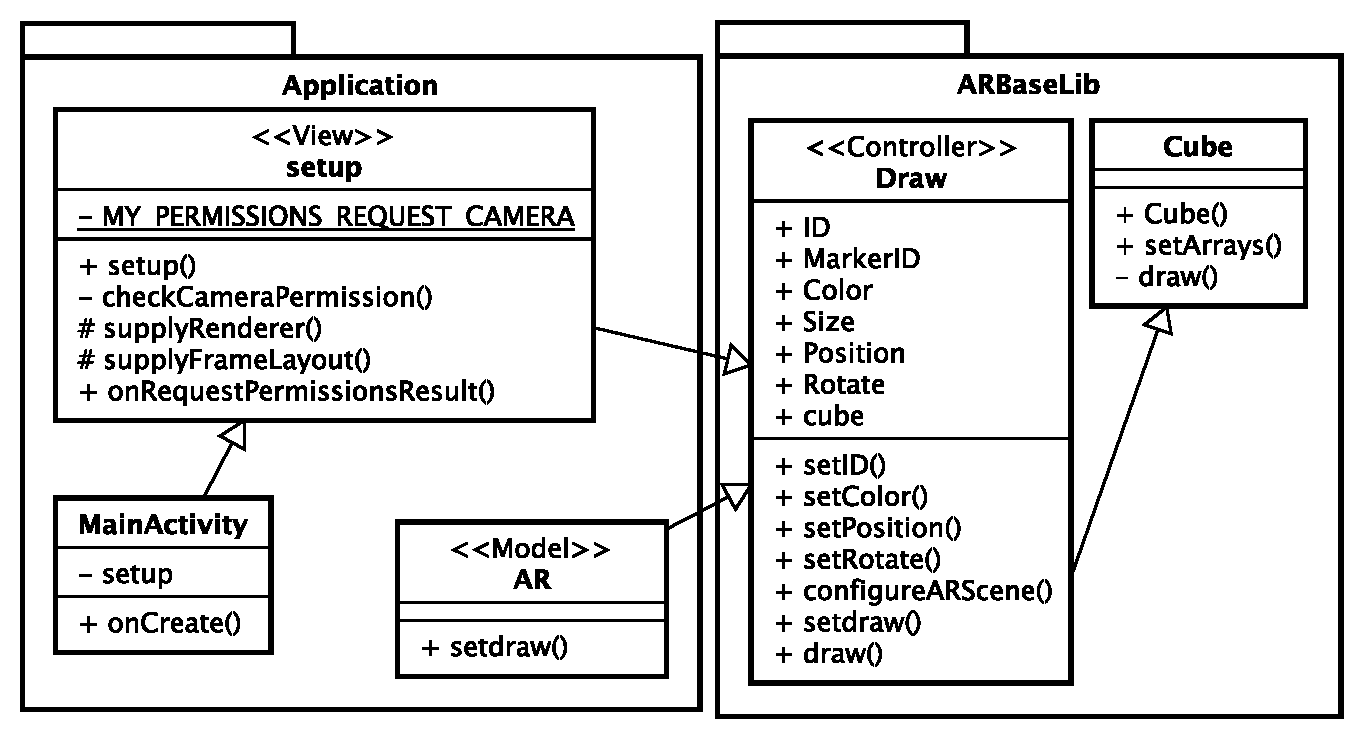
\includegraphics[width=12cm]{fig/android.pdf}
\caption{Class diagram}
\label{fig:class}
\end{figure}



\clearpage

%%%%% ----- 実装 ----- %%%%%
% [implement.tex]というTEXファイルを用意する
\section{実装}
\vspace{10pt}
前章で設計したクラスを実装する.
%\vspace{5pt}
\subsection{MainActivity}

\begin{itemize}
 \item 親クラスをSetupに変更し,onCreate\footnote{Androidアプリケーションが立ち上がる際に実行されるメソッド}内で親クラスのsetupメソッドを実行している.
 \item それ以外の処理は無く,アプリケーションを立ち上げた際に一度だけ呼ばれるクラスとなっている.
\end{itemize}

%\vspace{5pt}
\subsection{Setup}
\begin{itemize}
 \item 親クラスはARActivity\footnote{ARToolKitの中枢クラス,ライブラリのクラスを制御している}で,アプリの起動,画面の作成,カメラからの画像の取得など初期設定を全て担っている.またRenderer\footnote{3Dオブジェクトを描写するクラス}をセットするなど描写方面の初期設定も同時に担っている.
 \item 基本的にこのクラスは初期設定を担っている為中身を変更する事はない.よってライブラリに付属させて配布する事が可能である.
\end{itemize}

%\vspace{5pt}
\subsection{AR}
\begin{itemize}
 \item 後述するDrawクラスで描画するBoxの情報をSetするメソッドである.DrawクラスのSetterをまとめたクラスと言える.コードの内容もほぼDrawクラスのSetterを呼び出して数値を設定しているだけである.
 \item わざわざSetterだけを分離した理由は,変更箇所を一まとめにする事で変更してはいけないところを間違って変更してしまうなどのミスが減らせる事などである.
\end{itemize}

%\vspace{5pt}
\subsection{Draw}

\begin{itemize}
 \item 前述したARクラスから値を受け取るGetterと後述するCubeクラスで設定したBoxを描写するクラスである.ARクラスから受け取った値を元にCubeクラスでBoxを作成し,マーカー上に描写する.
 \item このDrawクラスの描写をするメソッドを変更する事で様々な表現が可能である.しかし今回のコンセプトは``とりあえず拡張現実感を体験しよう''なのでここではBoxを表示するだけにとどめている.
\end{itemize}

%\vspace{5pt}
\subsection{Cube}
\begin{itemize}
 \item 受け取った数値を元に大きさ,色,透明度の情報を持つBoxを生成するクラスである.
 \item ここを変更する事で様々な形を表現する事が可能である.また3Dオブジェクトの表示も可能である.しかし前述した通りコンセプトに合わない為Boxの表示をする機能だけにとどめた.
\end{itemize}

\subsection{実行結果}
実行結果をFig.\ref{fig:res1}~-~Fig.\ref{fig:res3}に示す.Fig.\ref{fig:res1}は実行前,Fig.\ref{fig:res2}は色指定が(R, G, B, α)の時\footnote{いずれも最大値は255である}(0, 255, 0, 0),Fig.\ref{fig:res3}は色指定が(0, 255, 255, 100)の時である.また使用者が実際に改変するクラスであるAR.javaを以下に示す.

\begin{lstlisting}
package com.example.yuut.test6;
import org.artoolkit.ar.base.Draw;

public class AR extends Draw{

	public Draw MarkerID = new Draw();

	@Override
	public void setdraw(){
		MarkerID.setID("single;Data/patt.hiro;80");
		MarkerID.setColor(0, 255, 255, 100);
		MarkerID.setSize(1);
	}
}
\end{lstlisting}

\begin{figure}[tb]
\centering
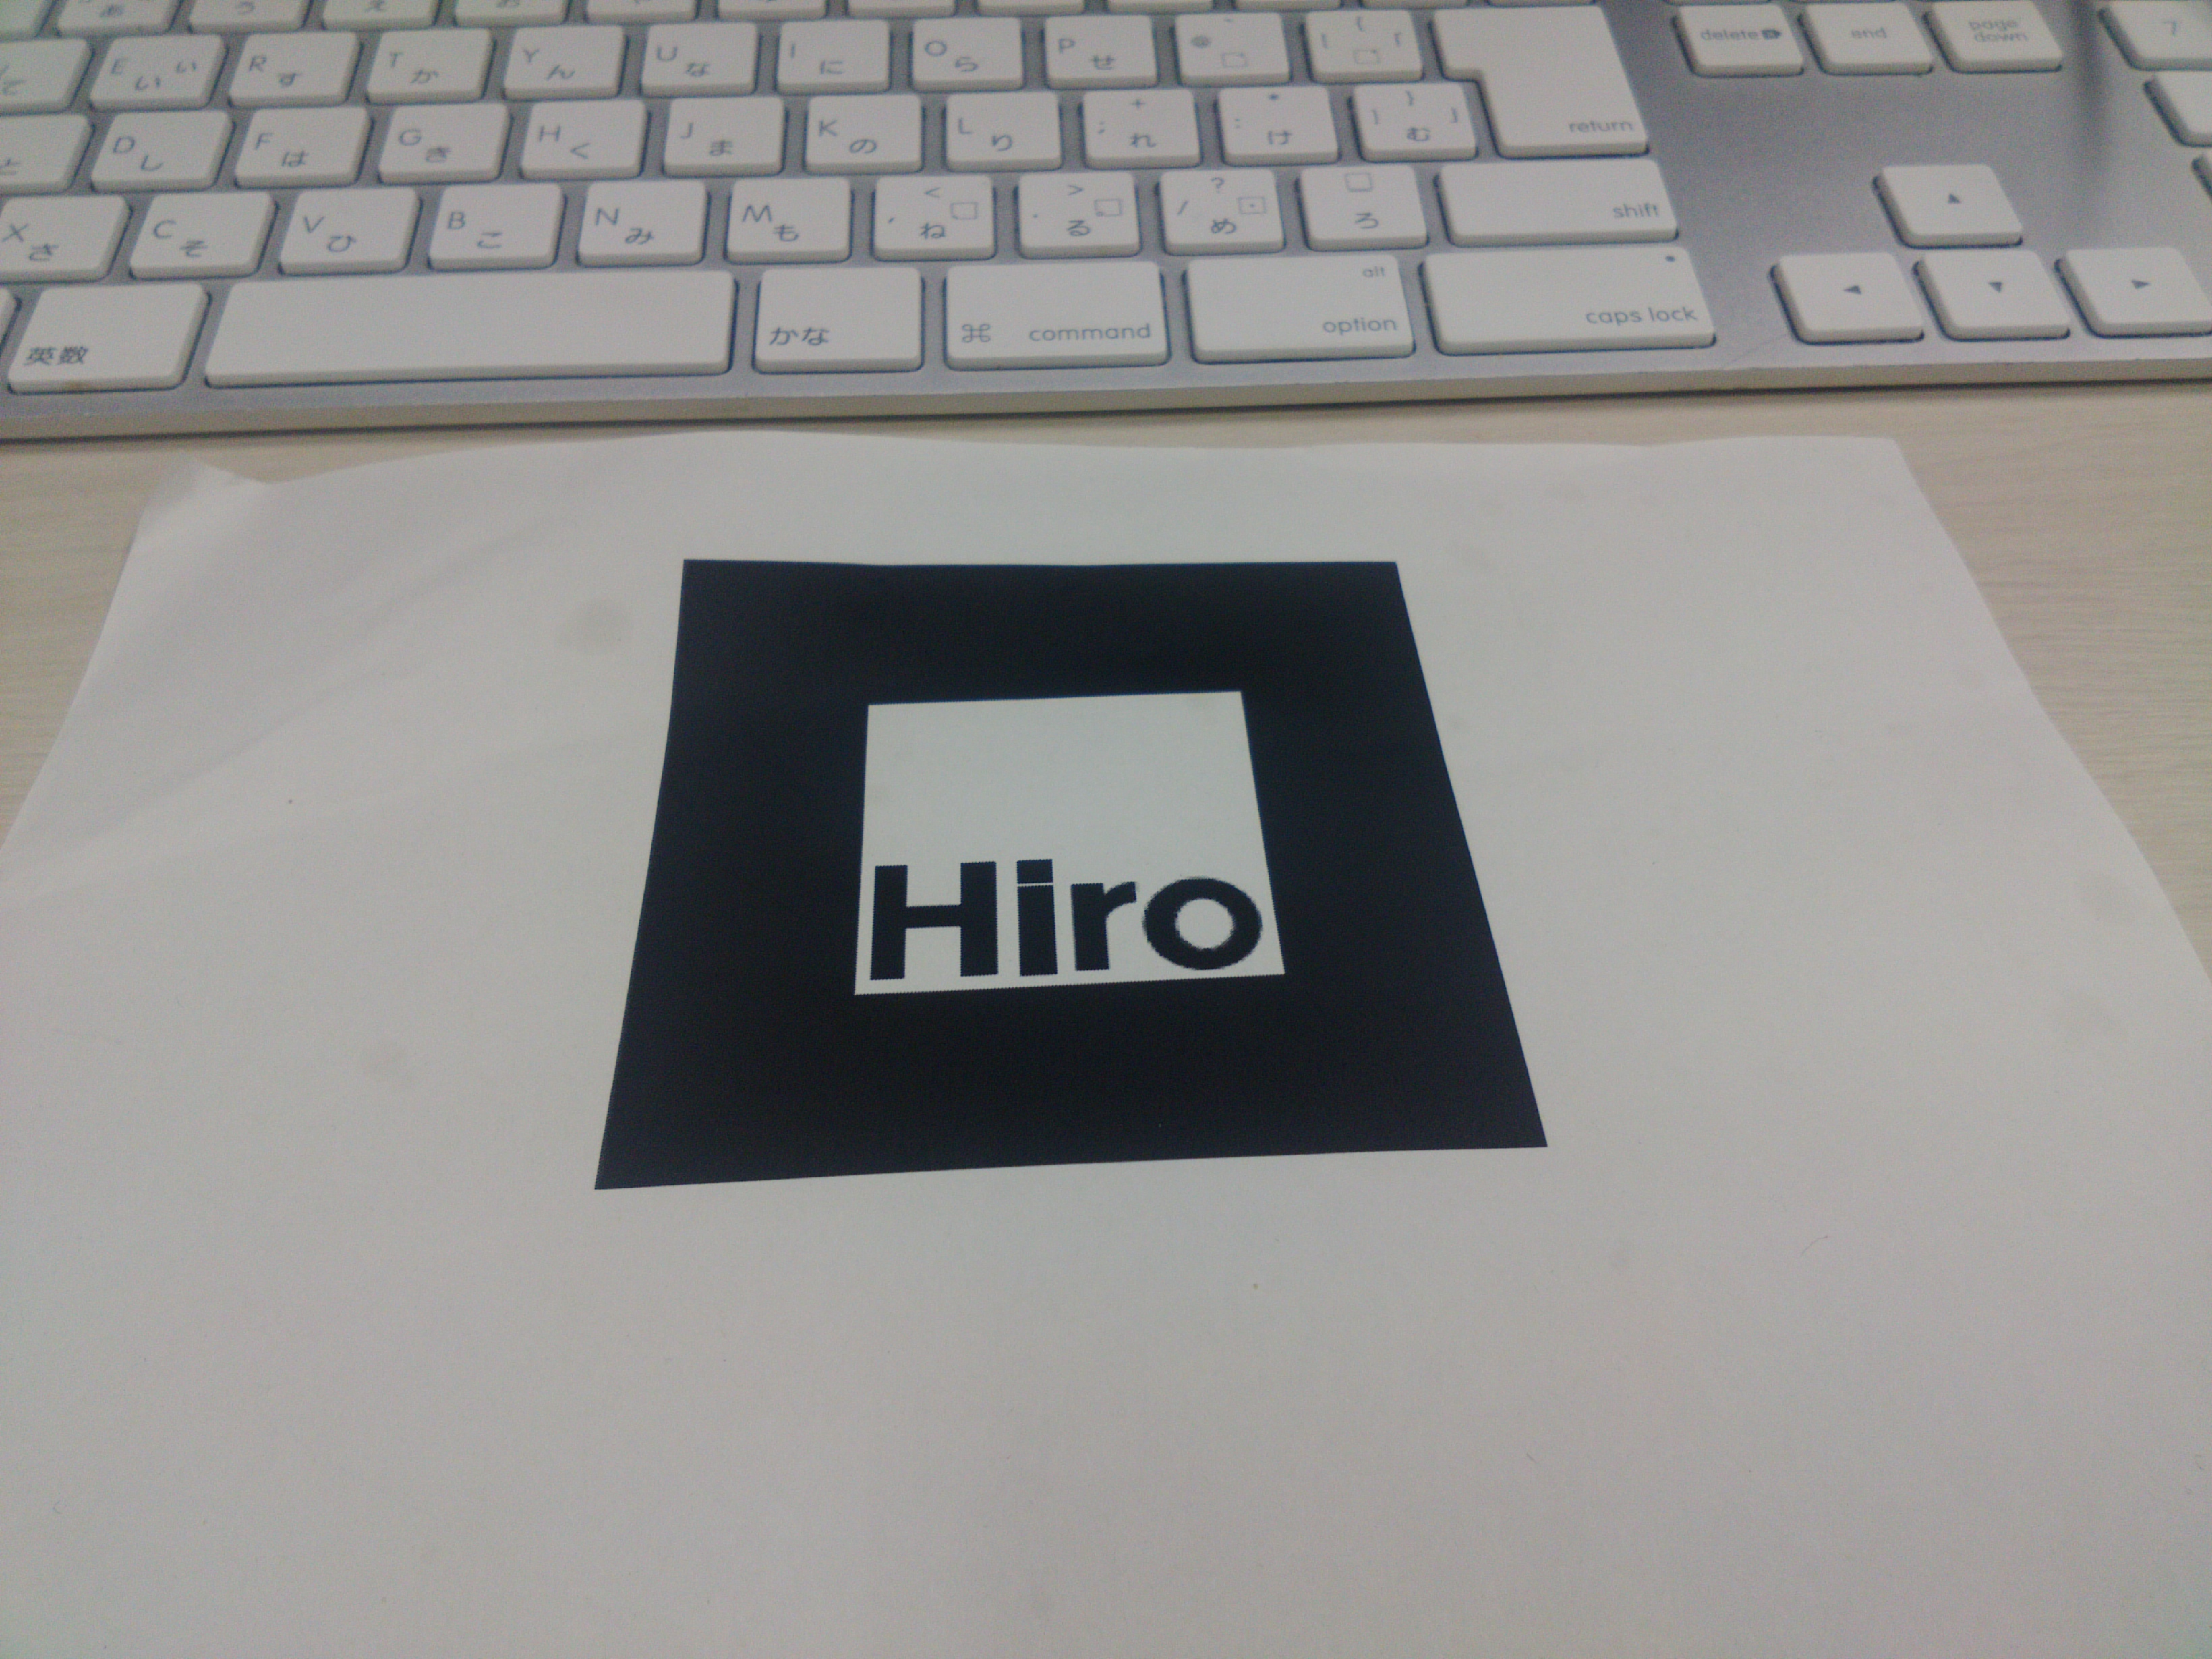
\includegraphics[width=9cm]{fig/res1.pdf}
\caption{Before execution}
\label{fig:res1}
\end{figure}
\begin{figure}[tb]
\centering
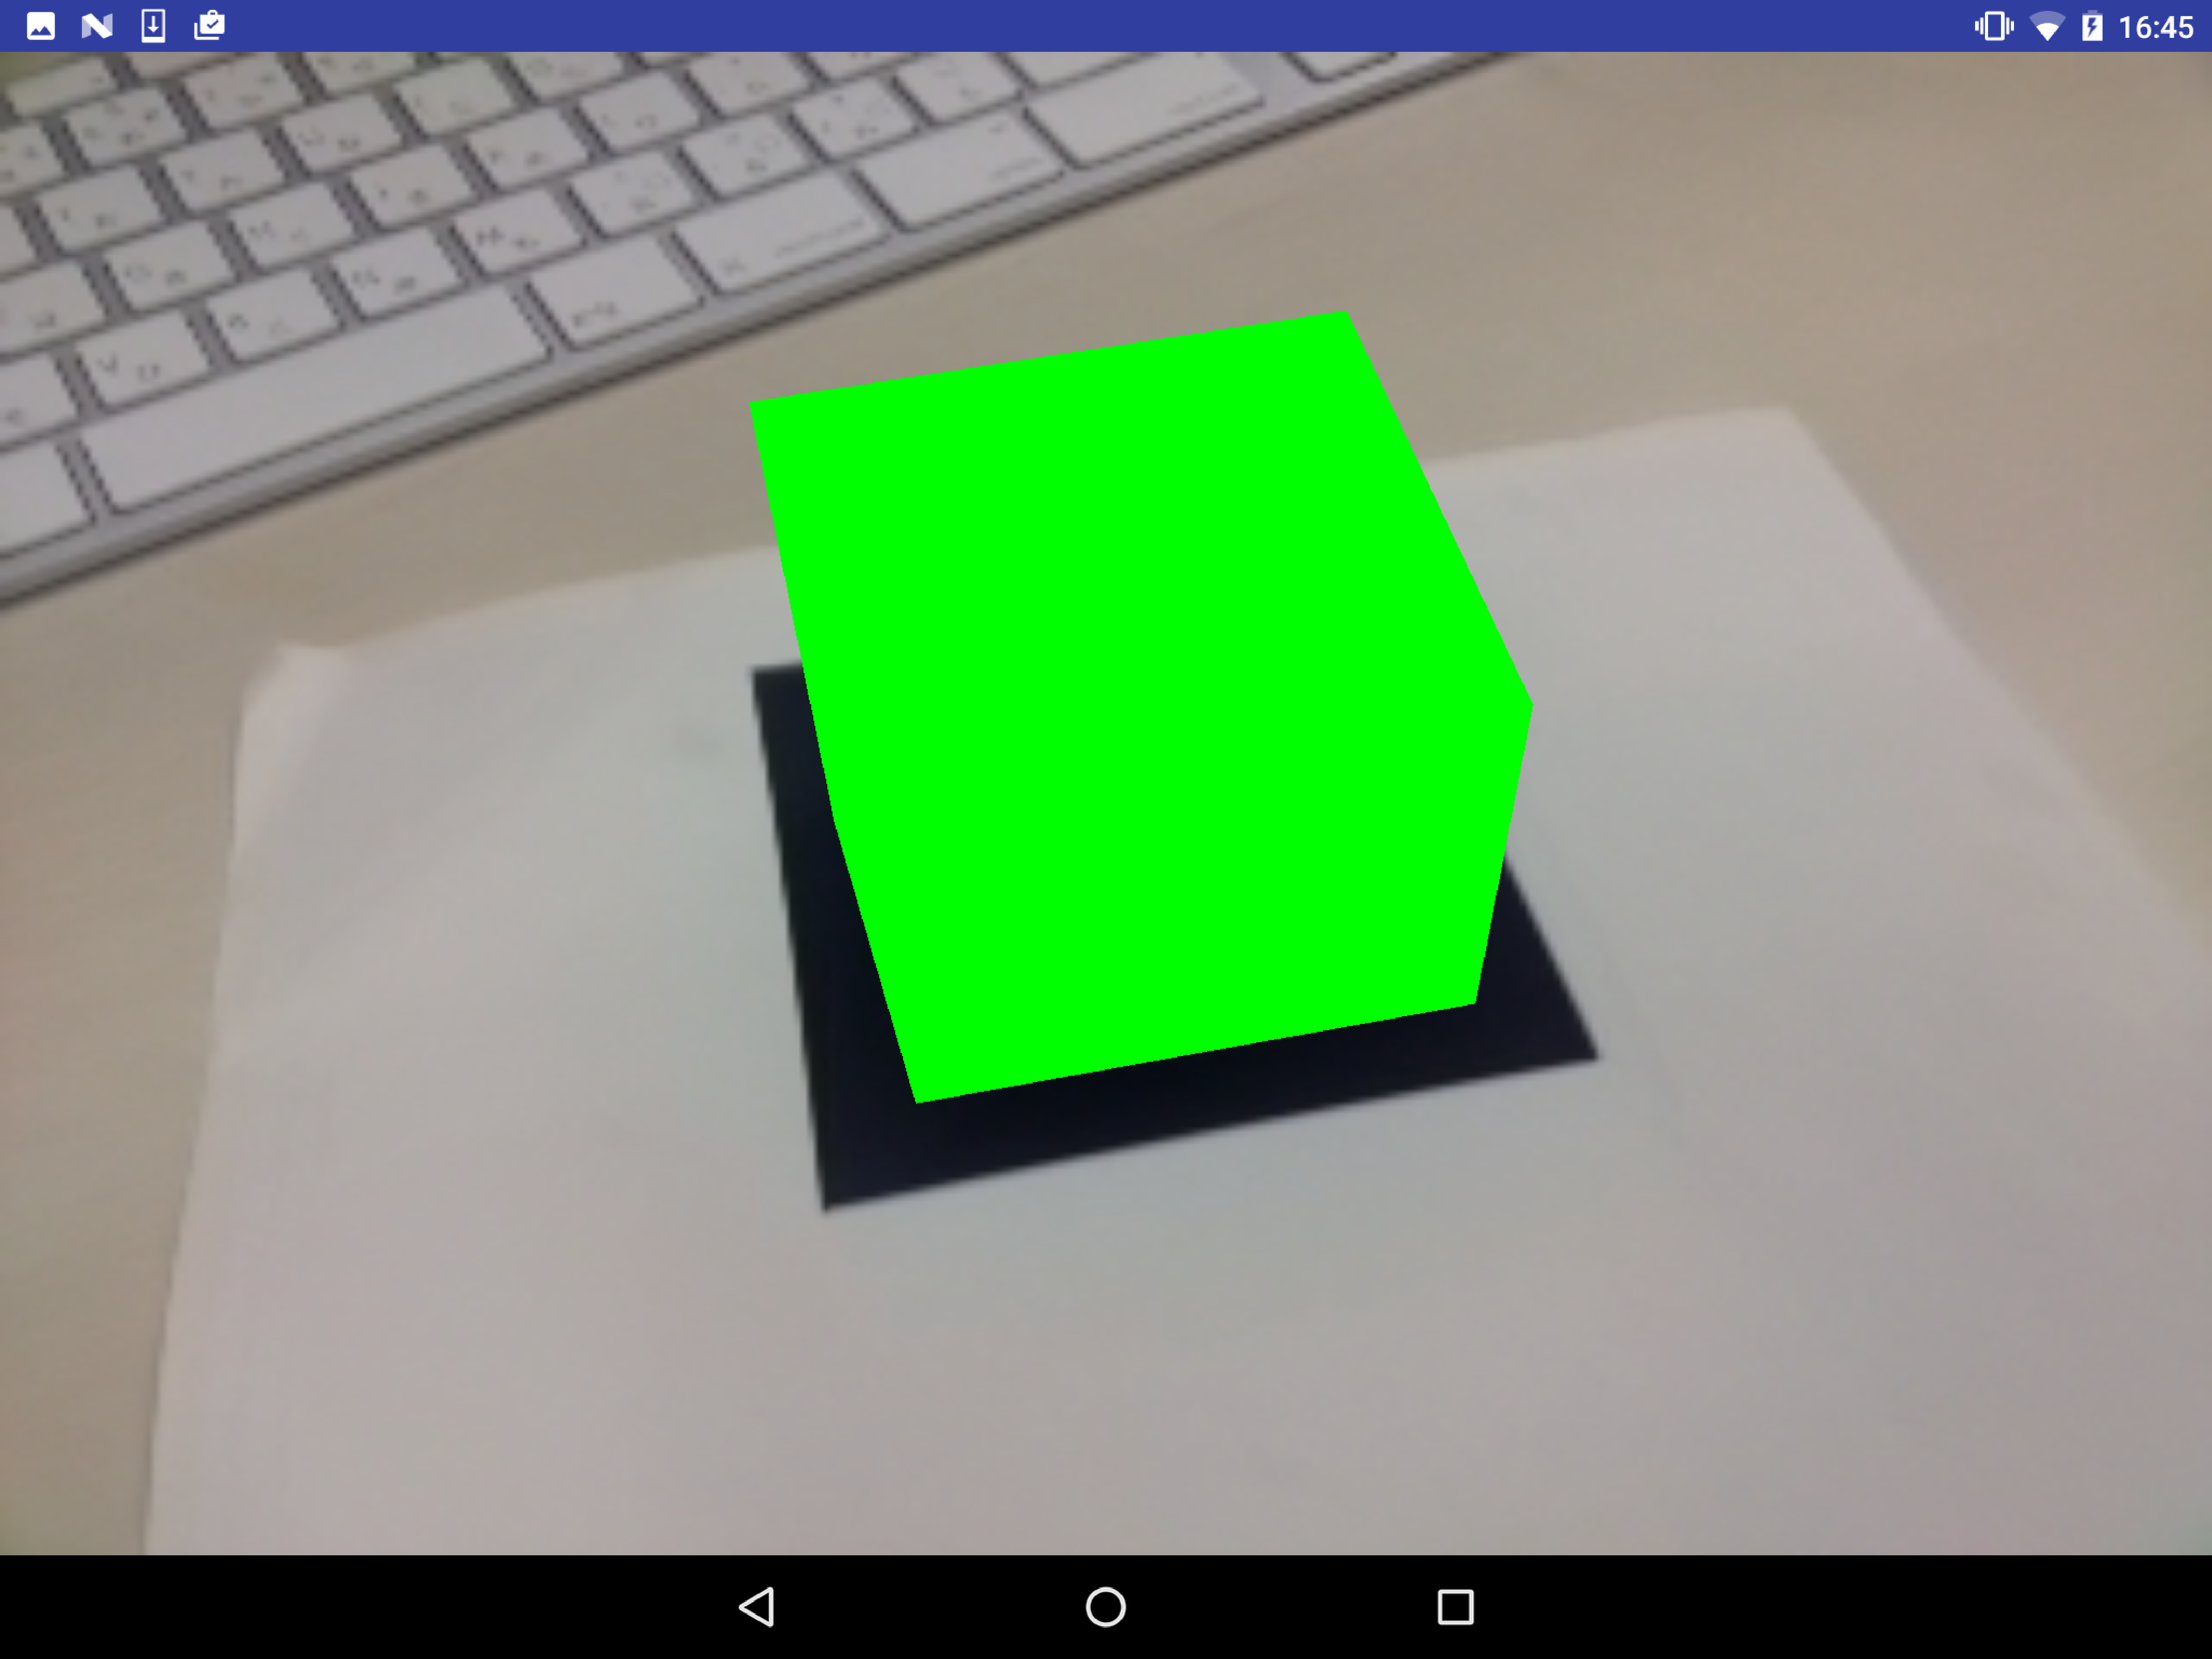
\includegraphics[width=9cm]{fig/res2.pdf}
\caption{Execution 1}
\label{fig:res2}
\end{figure}
\begin{figure}[tb]
\centering
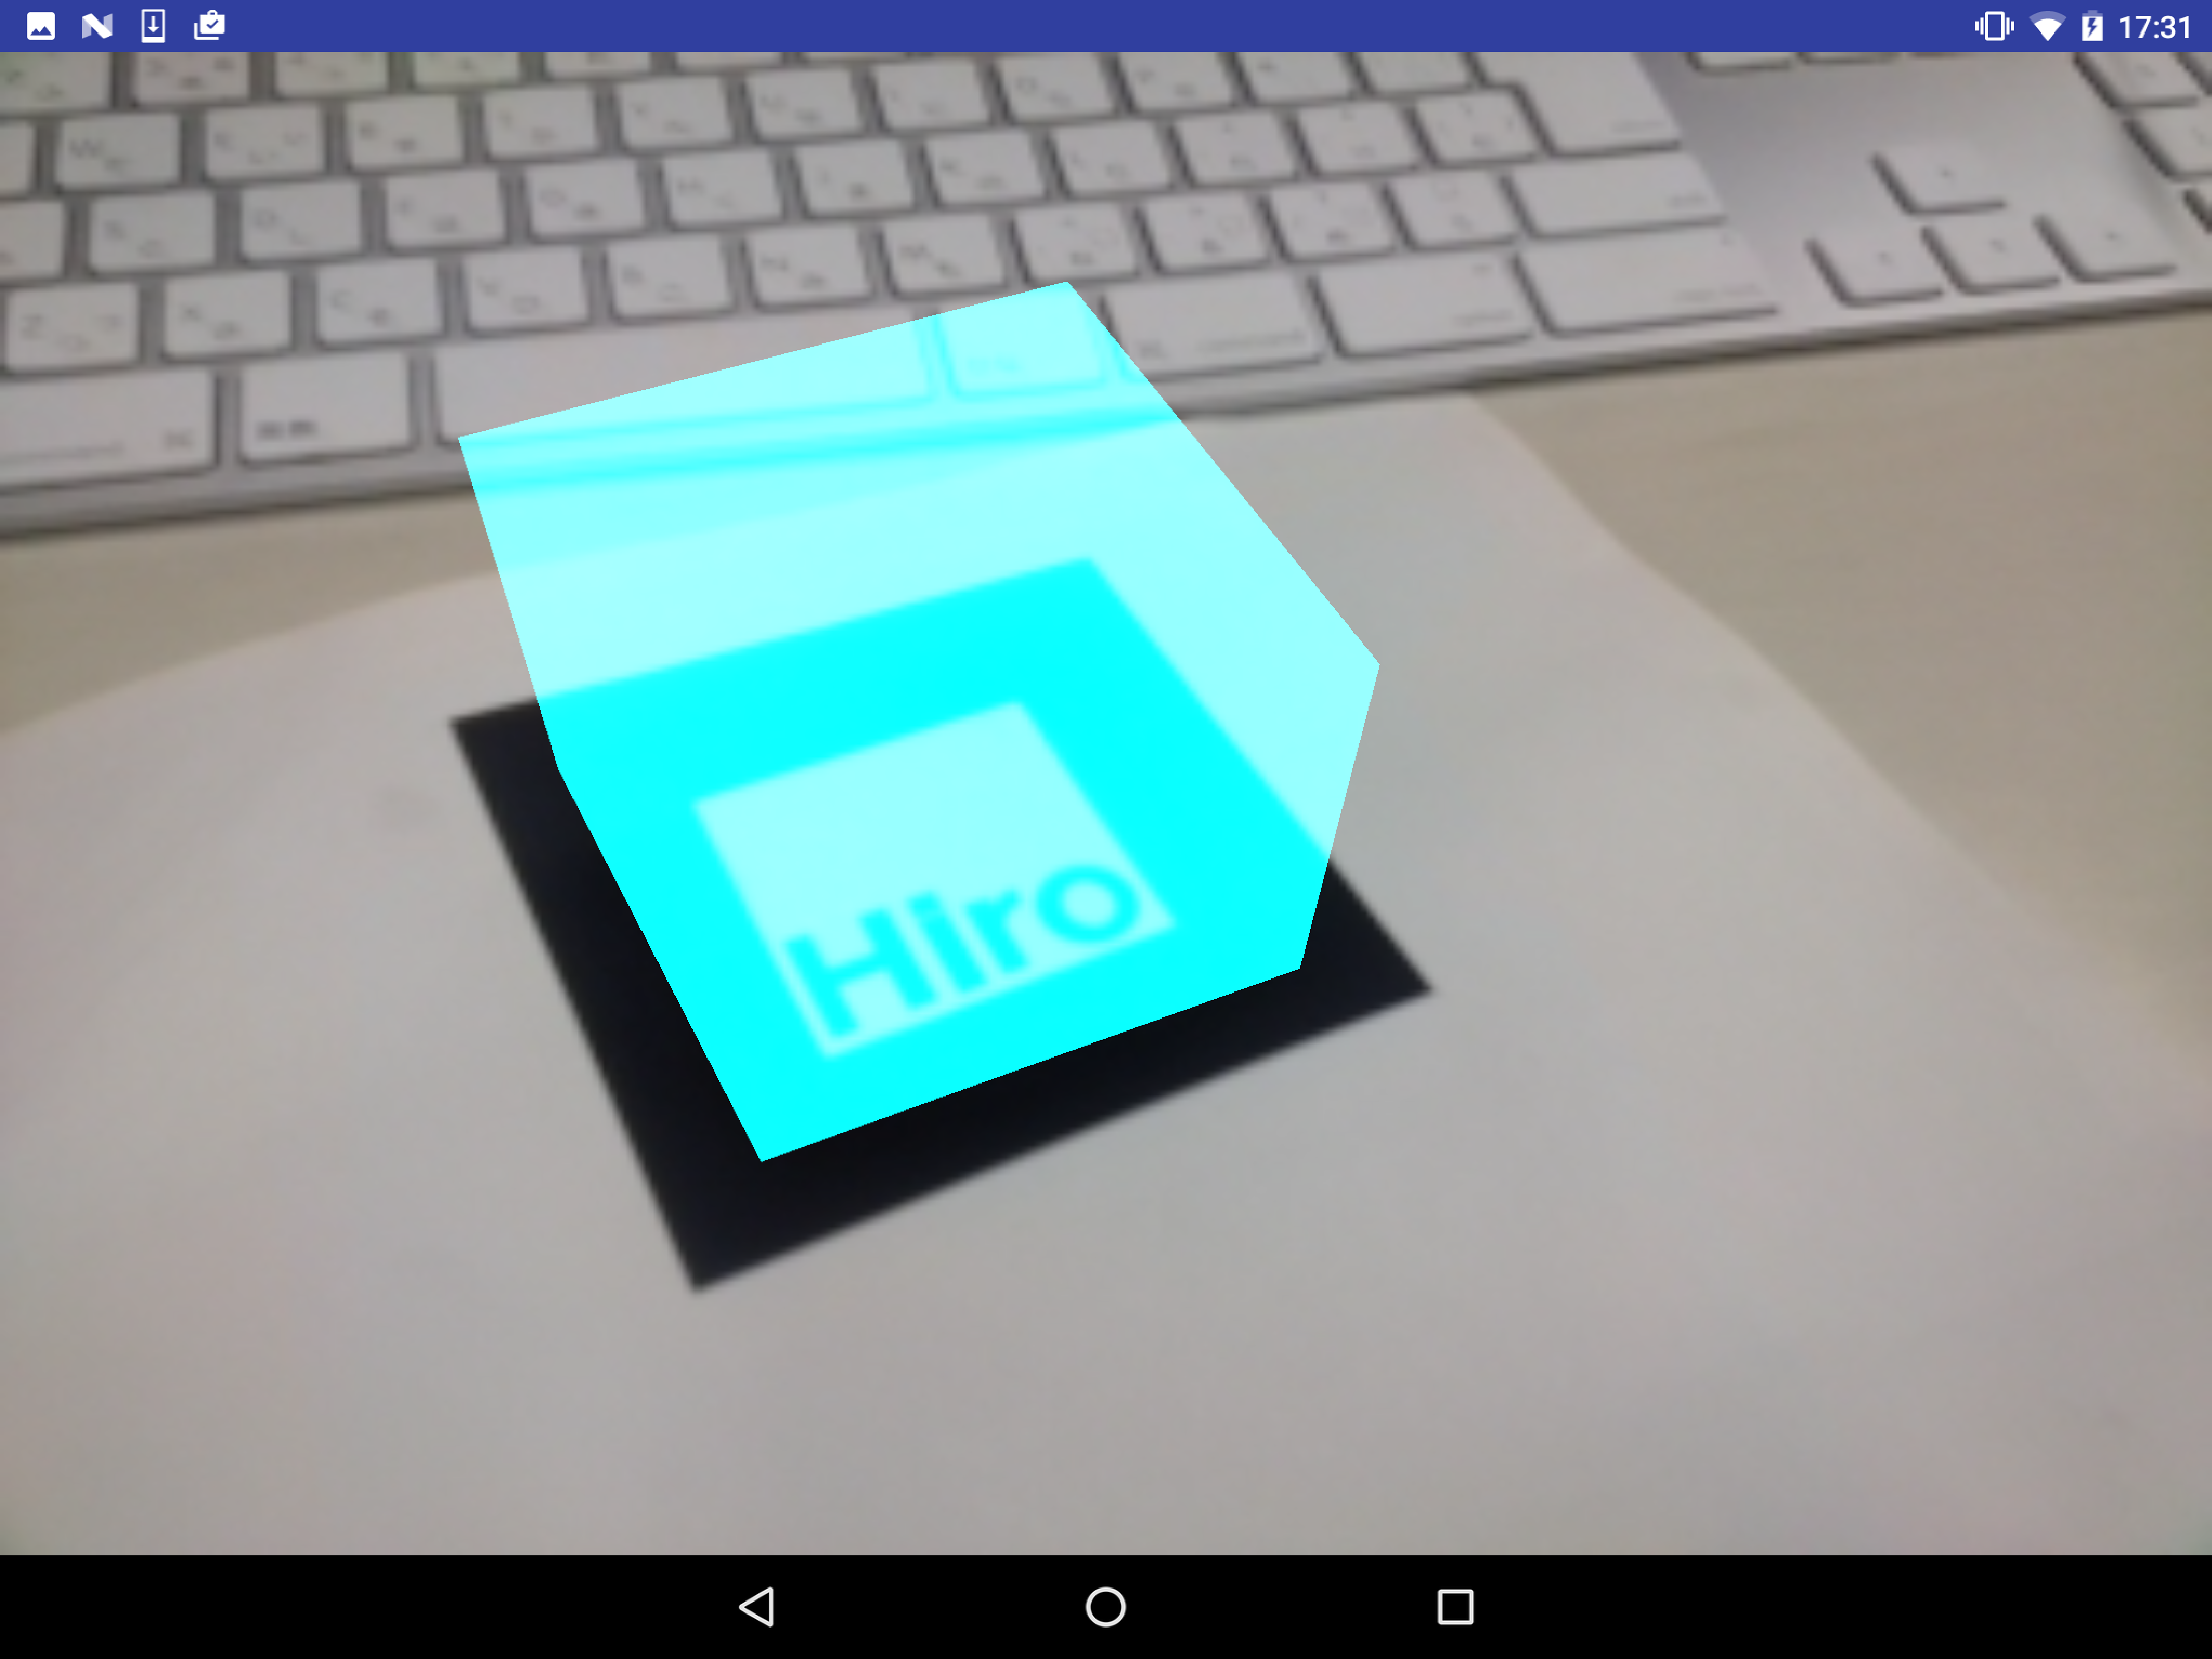
\includegraphics[width=9cm]{fig/res3.pdf}
\caption{Execution 2}
\label{fig:res3}
\end{figure}
\ 
\newpage
\clearpage

%%%%% ----- 検証 ----- %%%%%
% [verification.tex]というTEXファイルを用意する
\section{検証}
\vspace{10pt}
前章で実装したプログラムを実際に実行し,設定したコンセプトを達成できているか確かめる.
\vspace{5pt}
\subsection{関数名や変数名を明瞭化}
関数名や変数名を明瞭化する事によって拡張や改変する際にコードの役割が分かりやすくなる.
\begin{itemize}
	\item DrawやSetupなど,一目で何をするクラスなのかがよく分かるようになったと言える.ARクラスはそのままだと何をするクラスなのかが分かり辛いが,AR全般の設定をしている為このようなクラス名となった.
\end{itemize}
\vspace{5pt}
\subsection{各クラスの役割を明瞭化}
役割ごとにクラスを分ける事で,改変や拡張時にどこを変更するかがすぐに分かる.また改変時にエラーが生じた際,どこにエラーがあるかが分かりやすくなる.
\begin{itemize}
	\item MainActivity, Setup, AR, Draw, Cube等,クラスごとに役割を分け,何をするクラスなのかを明瞭化することが出来た.
\end{itemize}
\vspace{5pt}
\subsection{拡張しやすい構成に}
提供されたライブラリを使ってできることは限られており,またARを用いたAndroidプログラミングの学習用途であれば,拡張しやすい構成にすることは重要なことであると言える.
\begin{itemize}
	\item 拡張するにはライブラリ内を変更する必要があり,初学者には厳しいと考える.設計時の対象者では拡張は難しいだろう.拡張性については達成できたとは言い難い.
\end{itemize}
\vspace{5pt}
\subsection{MainActivityは最小限に}
MainActivityはCやJavaで言うMain関数である.Main関数は処理するクラスではなく,メソッドを実行するクラスであるため,ここでの処理は出来る限り最小限にすることが望ましい.
\begin{itemize}
	\item MainActivityはSetupクラスのsetupメソッドを呼び出すだけとなっている.その後はSetupクラスが初期設定をした後,ライブラリ内のARActivityが処理を引き継ぐ.
\end{itemize}
\clearpage

%%%%% ----- 考察 ----- %%%%%
% [consideration.tex]というTEXファイルを用意する
\section{考察}
\vspace{10pt}
開発したライブラリに対しての考察をする.
%\vspace{5pt}
\subsection{考察1 : Setupの複雑化}
まず第一に,Setupクラスについてである.このクラスはライブラリ内では出来ない設定をするクラスであり,ライブラリと共に提供されると説明したが,設計初期はこのクラスは存在せず全てライブラリ内で初期設定をする予定だった.しかし設計と並行してライブラリの学習をしていた際,どうしてもライブラリでは出来ない設定があることを知り,当初無かったこのクラスを実装することになった.しかし設計時の予想よりもライブラリでできる事は少なく,結果Setupクラスが膨大になってしまった.Setupクラスを提供する事によって実装時の負担を減らすことが出来たが,分かりやすいライブラリからは少し遠ざかってしまった.後述するがここは今後の一番の課題であると考える.

%\vspace{5pt}
\subsection{考察2 : 拡張性}
第二に,拡張性についてである.前述したとおり,拡張性については達成できたとは言い難い.その原因として,簡易化するにあたって内部処理の大半をライブラリ内に格納してしまったからであると考える.これは拡張性と簡易化がトレード・オフの関係にあると言え,拡張性を求めると今度は簡易化が達成できない.しかし簡易化すると今度は拡張性が失われる.この二つを両立させることは難しいが,拡張する範囲を限定することで両立に近づけることはできるだろう.この場合どの範囲まで拡張性をもたせるかの判断も必要であり,後述する課題の一つと考えることができる.またライブラリ内の構成を工夫することでライブラリの改変を簡易化することができれば拡張性を失うことなく簡易かも達成できるだろうと考える.

%\vspace{5pt}
\subsection{考察3 : MainActivity}
第三に,MainActivityである.今回は親クラスを変更したが,MainActivityは所謂Mainクラスであるため,親クラスを変更することは望ましくない.既存のプログラムでMainActivityを既に改変していた際,本ライブラリの導入が出来ない可能性があるからだ.今回はARの体験,というコンセプトだった為,既存プログラムへの導入に関しては想定には含まなかったが,今後ライブラリを改良していく際の課題の一つであると考える.
\clearpage

%%%%% ----- 総評 ----- %%%%%
% [asess.tex]というTEXファイルを用意する
\section{総評}
\vspace{10pt}
実装したライブラリの評価,課題及び今後の発展について,以下に述べる.
\vspace{5pt}
\subsection{評価}
実装したライブラリの検証,及び考察から,設計時のコンセプトは概ね実現していると言える.実際ARクラスを変更するだけで様々なBoxを表示することができるようになった.これによりARとはどんなものなのか,またAndroidでARを動かすために必要な処理がどんなものなのか等の学習に適切なライブラリになったと言えるだろう.またAndroudStudioの設定やライブラリの導入などを事前にしておけば中学生でもAndroidでARを動かすことができるだろう.

\vspace{5pt}
\subsection{課題}
検証及び考察で述べた通り,以下の課題が残っている.

\vspace{5pt}
\subsubsection{Setupの簡易化及びライブラリ内への格納}
先述した,今後一番の課題である.Setupクラスでは初学者には難しい初期設定などが記述されており,記述するにはとても難易度が高いものである.今回はライブラリと共に提供という形になったが,ライブラリ内に格納できればそのような問題はなくなる.この課題が達成できれば,Appモジュール内はMainActivity及びARクラスの二つのみとなり,使用者の作業が格段に簡易化される.ここまで簡易化されれば,プログラム未経験者対象のセミナーなどでARを体験することも容易になるだろう.

\vspace{5pt}
\subsubsection{拡張性の確保}
先述したが,拡張性は簡易化とトレード・オフの関係にありライブラリの簡易化は拡張性の喪失とも言える.しかしライブラリ内を更に簡易化し段階的に拡張性をもたせれば拡張性を喪失せずに簡易化できると考える.Appモジュール内の変更,ライブラリ内の変更,この二つを段階的にすれば拡張性をもたせつつ簡易化できるだろう.

\newpage
\subsubsection{MainActivityの親クラスの変更}
MainActivityの親クラスの変更は既存プログラムへの組み込みには適さない.この問題はSetupの簡易化及びライブラリ内への格納の問題が解決すると同じく解決するため,並行して進めていく予定である.

%\vspace{5pt}
\subsection{今後の発展}
本ライブラリを更に改良することで更に簡易化し,また拡張性をもたせ様々な人にとって使いやすいものにしようと考えている.また以下の機能を追加することで更にARについて学べるライブラリになると考えている.

\begin{itemize}
 \item 3Dオブジェクトの表示
 \item 時間経過による変化の組み込み
 \item 複数マーカの認識
 \item テキストの表示
 \item 画像,動画の表示
\end{itemize}

以上の機能を簡易化し,組み合わせやすくすることで今後の情報教育にも十分活用できるライブラリになると考える.
\clearpage

%%%%% ----- おわりに ----- %%%%%
% [final.tex]というTEXファイルを用意する
\section{おわりに}
\vspace{10pt}
本ライブラリによってAndroidアプリケーション開発初学者でも,比較的簡単に拡張現実感を体験する事ができるようになったと考える.ディスプレイを見ながらカメラを動かすのではなく,カメラの視点と自分の視点がほぼ同じで直感的な操作ができる点でAndroidはとても有用であり,今後の発展も望めるだろう.しかし課題も多くまだ実用的だとは言い難い.今後の発展で述べたもの以外にも,Raspberry Piとの連携など,更に拡張現実感の入門用ライブラリとしての十分な機能を実装したい.%\par
%\vspace{5pt}

拡張現実感ははじめに述べたように遊戯ではなく生活の補助として発展するだろうと予測している.車,テレビ,冷蔵庫などの登場,携帯電話の登場,スマートフォンの登場と,今までの生活が大きく変わる発明が過去に沢山あった.拡張現実感を用いた製品の登場が今までの生活を大きく変えるものとなるかどうかはまだ分からないが,大きく期待はしている.

%\par \vspace{5pt}
ヘッドマウントディスプレイ(HMD)と言うものがある.これは頭に装着して拡張現実感の出力先として使用する装置である.今はまだ機械自体が大きく,これを着けて外を歩くのは実用的ではない.しかし日本の得意分野である小型化によって簡単に外に持ち運べるようなものになった時,生活が大きく変わるだろうと考えている.また,スマートグラスという外見が眼鏡のようなものも数多く登場しており,拡張現実感の出力先の発展は遅れながらも確実に進んでいる.

%\par \vspace{5pt}
出力先の発展だけでは拡張現実感は発展しない.本研究のようなARライブラリの開発も必要不可欠である.今後,更にたくさんのARライブラリの開発が進むことを願っている.
最後に,本ライブラリによって更に拡張現実感に触れる機会が増え,興味を持っていただける事を期待している.
\clearpage

%%%%% ----- 謝辞 ----- %%%%%
% [thanks.tex]というTEXファイルを用意する
\section{謝辞}
\vspace{10pt}
本研究を進めるにあたり,拡張現実感や開発基盤に関する多大な知識をご教授頂いた指導教員の小飼敬先生に感謝します.また,英文テーマの決定及びライブラリ開発の際に生じた疑問についてご教授頂いた石垣達也先生に感謝します.最後に,この一年間協力してくれた小飼研究室のメンバに感謝します.
\par \vspace{5pt}
ここから先は削除してね.ここでは1年間で協力してくれた方に謝辞を述べるところです.間違っても研究に関係のない人を書かないように(恋人とか書いてると将来黒歴史になるので注意)\\
最初に担当教員,そのあとは研究室から遠い順に.例えば...\\

\begin{itemize}
 \item 担当教員
 \item 学校外の協力者
 \item 他学科の協力者
 \item 学科内の先生
 \item 学科外の生徒
 \item 学科内の生徒
\end{itemize}

学科外の生徒を学科内の先生より先に書くかどうかは私もよくわかりません.そこまでたくさん書く必要はないです.
\clearpage

%%%%% ----- 参考文献 ----- %%%%%
% [reference.tex]というTEXファイルを用意する
\vspace{10pt}
\begin{thebibliography}{99}
	\bibitem{タグをここに書く} 会社名や人物名 - サイト名や書籍名\\ アドレスや出版社
	\bibitem{VR} 日本バーチャルリアリティ学会 - バーチャルリアリティとは\\ https://vrsj.org/about/virtualreality/
	\bibitem{VRnews} Engadget日本版 - 「PlayStation VR」1月26日に再販スタート、同日発売の「バイオハザード7」もVR完全対応\\ http://japanese.engadget.com/2017/01/16/playstation-vr-1-26-7-vr/
	\bibitem{ARapp} KDDI - 「ARナビゲーション」機能追加について\\ http://www.kddi.com/corporate/news\_release/2013/0117/besshi2.html
	\bibitem{SG} Weblio辞書 - スマートグラス\\ http://www.weblio.jp/content/スマートグラス
	\bibitem{ARnavi} Pionner - サイバーナビ\\ http://pioneer.jp/carrozzeria/cybernavi/avic-vh99hud\_avic-zh99hud/
	\bibitem{ARToolKit} ARToolKit - Android Documentaion\\ http://artoolkit.org/documentation/doku.php?id=4 Android:android about
	\bibitem{NyARToolkit} NyARToolkit project - Welcome to NyARToolkit project\\ http://nyatla.jp/nyartoolkit/wp/
	\bibitem{AndAR} Google Code - AndAR Android Augmented Reality\\ https://code.google.com/archive/p/andar/
	\bibitem{Processing} Processing - Cover\\ https://processing.org/
	\bibitem{Eclipse} Eclipse - MainPage\\ https://eclipse.org/
	\bibitem{AndroidStudio} Android Developers Site - Android Studio\\ https://developer.android.com/studio/intro/index.html
	\bibitem{Yosemite} Apple - OS X Yosemite (2014年 10月 22日 INTERNET ARCHIVE - WayBack Machine)\\ http://web.archive.org/web/20141022105913/http://www.apple.com/jp/osx/
	\bibitem{Nexus9} HTC - Nexus 9\\ http://www.htc.com/jp/tablets/nexus-9/
\end{thebibliography}
\clearpage

%%%%% ----- 付録 ----- %%%%%
% [appendix.tex]というTEXファイルを用意する
\appendix
\section{付録名}
\vspace{10pt}
付録をここに書く

\end{document}